\subsection{CaloChallenge 2022}
{{\footnotesize
\noindent The Fast Calorimeter Simulation Challenge 2022 assessed 31 generative-model submissions (VAEs, GANs, Flows, Diffusion)
on four calorimeter shower datasets; benchmarking shower quality, generation speed, and model complexity .


\begin{description}[labelwidth=4cm, labelsep=1em, leftmargin=4cm, itemsep=0.1em, parsep=0em]
  \item[date:] 2024-10-28
  \item[version:] v1.0
  \item[last\_updated:] 2024-10
  \item[expired:] unknown
  \item[valid:] yes
  \item[valid\_date:] 2024-10-28
  \item[url:] \href{http://arxiv.org/abs/2410.21611}{http://arxiv.org/abs/2410.21611}
  \item[doi:] 10.48550/arXiv.2410.21611
  \item[domain:] LHC Calorimeter; Particle Physics
  \item[focus:] Fast generative-model-based calorimeter shower simulation evaluation
  \item[keywords:]
    - calorimeter simulation
    - generative models
    - surrogate modeling
    - LHC
    - fast simulation
  \item[licensing:] Via Fermilab
  \item[task\_types:]
    - Surrogate modeling
  \item[ai\_capability\_measured:]
    - Simulation fidelity
    - speed
    - efficiency
  \item[metrics:]
    - Histogram similarity
    - Classifier AUC
    - Generation latency
  \item[models:]
    - VAE variants
    - GAN variants
    - Normalizing flows
    - Diffusion models
  \item[ml\_motif:]
    - Surrogate
  \item[type:] Dataset
  \item[ml\_task:]
    - Surrogate Modeling
  \item[solutions:] Solution details are described in the referenced paper or repository.
  \item[notes:] The most comprehensive survey to date on ML-based calorimeter simulation; 31 submissions over different dataset sizes.

  \item[contact.name:] Claudius Krause (CaloChallenge Lead)
  \item[contact.email:] unknown
  \item[datasets.links.name:] Four LHC calorimeter shower datasets
  \item[datasets.links.url:] \href{various voxel resolutions}{various voxel resolutions}
  \item[results.links.name:] ChatGPT LLM
  \item[fair.reproducible:] Yes
  \item[fair.benchmark\_ready:] Yes
  \item[id:] calochallenge\_
  \item[Citations:] \cite{krause2024calochallenge2022communitychallenge}
\end{description}

{\bf Ratings:} ~ \\

\begin{tabular}{p{0.15\textwidth} p{0.07\textwidth} p{0.7\textwidth}}
\hline
Rating & Value & Reason \\
\hline
dataset & 5 & Four well-structured calorimeter datasets are provided, with different voxel resolutions,
open access, signal/background separation, and metadata. FAIR principles are well covered.
 \\
documentation & 4 & Accompanied by a detailed paper and dataset description. Reproduction of pipelines may require
additional setup or familiarity with the model submissions.
 \\
metrics & 5 & Metrics like histogram similarity, classifier AUC, and generation latency are well defined
and relevant for simulation quality, fidelity, and performance.
 \\
reference\_solution & 4 & Several baselines (GANs, VAEs, flows, diffusion models) are documented and evaluated.
Some are available via community repos, though not all are fully standardized or bundled.
 \\
software & 4 & Community GitHub repos and model implementations are available for the 31 submissions.
While not fully unified in one place, the software is accessible and reproducible.
 \\
specification & 5 & The task—evaluating fast generative calorimeter simulations—is clearly defined with
benchmarking protocols, constraints like latency and model complexity, and structured
evaluation criteria.
 \\
\hline
\end{tabular}

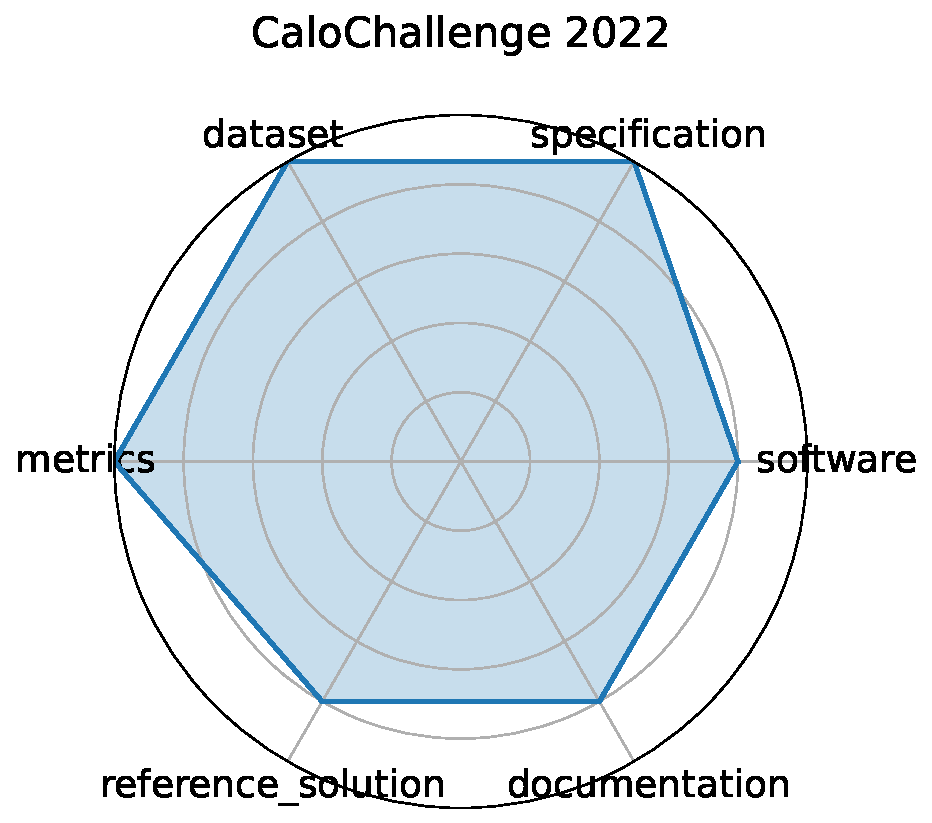
\includegraphics[width=0.2\textwidth]{calochallenge__radar.pdf}
}}
\clearpage